\section{Unary Color Properties}
\label{sec:unary}

\remark{Introduction (Why do we need these terms?)}

\remark{List all the properties we model, giving rationale for including each one}

\remark{We model these properties for both individual segments and for groups. Explain rationale}

\remark{List all the predictive features we use, both for groups and segments, and give rationale}

\remark{Give the form of the function phi, for a single group (and single segment)}

\remark{Show an example of two regions that have different feature vectors \& different predicted CPDs for some property (Perhaps background colorfulness vs. foreground colorfulness?)}

\remark{Finally, talk about how we learn these distributions from data (subsection)}

As shown in Figure~\ref{fig:ColorCompatOnly}, color compatibility alone does not predict attractive colorings. Good color assignments also depend on the properties of the regions being colored and their spatial arrangement. To capture these dependencies, our model includes spatial terms over groups, segments, and segment adjacencies in the pattern. Group and segment terms capture color dependencies on region features, and segment adjacency terms capture color dependencies on the relationship between nearby regions.

These spatial terms score color assignments based on the conditional probability of a color property $\prop$ (such as lightness or colorfulness) given the features of an object $x$ (which is either a group, segment, or segment adjacency). We compute these probabilities on color properties instead of directly on colors to allow for more generalization over colors that do not occur in the model's training data. For example, Figure~\ref{fig:conditionalDistribution} shows the conditional probability distribution over lightness for the background group of one pattern. The distribution is conditional on several characteristic features of the group, such as its size and the number of segments it contains. In the next sections, we give definitions for the group and segment terms in the model and the adjacency terms. We then describe how to learn these conditional probability distributions from example patterns (Section~\ref{sec:learningPdfs}). A complete listing of the features used, as well as more details on the computation of color properties, can be found in the Appendix.

\begin{figure}[ht]
\begin{tabular}{cc}
\raisebox{5em}{
\includegraphics[width=.22\columnwidth]{figs/histogramImage}}&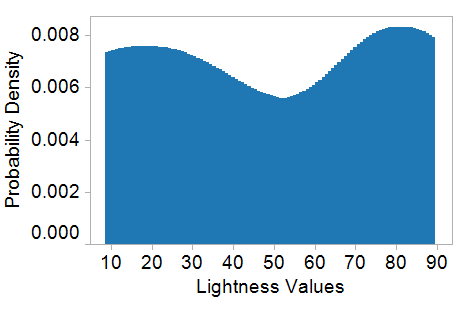
\includegraphics[width=.7\columnwidth]{figs/histogram}%\vspace{0.5em}\\
\end{tabular}
\caption{The conditional probability distribution of lightness values for the background color group of a pattern (highlighted in orange). The distribution's multimodality indicates that either very light or very dark backgrounds may be acceptable for this pattern.}
\label{fig:conditionalDistribution}
\end{figure}

Both global group features as well as local segment features affect the appearance of a color assignment. The total area of a group and overall spread of its member segments correspond to the overall proportion and spread of its assigned color within an image. In addition, the size and shape of member segments may impact the color a group takes on. As an example, smaller segments may often be more saturated, and a group composed of many small segments may be more likely to be saturated than a group composed of a few small segments but also one large segment \remark{S: Made up example. Should probably find one that holds in our data}.

Our model has one group and one segment term for each of the color properties $ \prop \in \unaryProps$, which are \propName{Lightness}, \propName{Colorfulness}, \propName{NameCounts}, and \propName{NameSaliency}.
The properties \propName{Lightness} and \propName{Colorfulness} are computed in \lab space. \propName{NameCounts} (counts of how many times a color is described with different names) and \propName{NameSaliency} (how uniquely a color is named) are as described by Heer and Stone~\shortcite{ColorNamingModels}. While lightness and colorfulness capture perceptual properties of color, name saliency and color name counts capture more categorical properties.

The group term for property $\prop \in \unaryProps$ has the statistic:
\begin{align*}
 \groupTerm(\colors|\pattern) &= \sum_{\group \in \groups} \groupInstStats(\colors_\group | \pattern, \group) \\
 \groupInstStats(\colors_\group | \pattern, \group) &=  \ln p( \prop( \colors_\group ) | \features_\group ) \cdot \size_\group
\end{align*}
where $\size_\group$ is the area of the group $\group$ and $\features_\group$ are the features of the group $\group$ (See the Appendix for the complete list of features used). We weight the contribution of each group to the term statistics by its relative area as larger regions tend to have more impact on the appearance of a coloring.

Similarly, the segment term for property $\prop$ has the statistics function $\segTerm(\colors|\pattern) = \sum_{\segment \in \segments} \segInstStats(\colors_\segment | \pattern, \segment)$, where $\segInstStats(\colors_\segment | \pattern, \segment) = \ln p( \prop( \colors_\segment ) | \features_\segment) \cdot \size_\segment$. Here, $\size_\segment$ is the size of the segment $\segment$ and $\features_\segment$ are the features of $\segment$.

These terms contribute unary factors over each color variable by grouping together statistics for the group and segments associated with the variable:
\begin{align*}
 \factor(\colorVars_\group | \pattern) = \prod_{\prop \in \unaryProps}
 		\exp( (&\groupTermWeight \cdot \groupInstStats(\colorVars_\group | \pattern, \group)  \\
 		     + &\segTermWeight \cdot \sum_{\segment \in \group} \segInstStats(\colorVars_\group | \pattern, \segment))) 
\end{align*}

\subsection{Learning Conditional Probability Distributions}
\label{sec:learningPdfs}

Each group, segment, and adjacency term requires a conditional probability distribution $p(\prop(\colorVars_x)|\features_x)$ in order to compute its statistic value. What form should these distributions take? Closed-form continuous distributions, such as the normal distribution, are appealing for their simplicity.  However, they are unlikely to capture the nuances of data drawn from real patterns, which is often \emph{multimodal} in nature. As a simple example, pattern backgrounds are typically either very dark or very light (See Figure~\ref{fig:conditionalDistribution}). A normal distribution cannot faithfully capture this type of bimodal behavior.

In our model, we adapt the method of Charpiat et al.~\shortcite{MultimodalColorization}, who learn conditional probability distributions of colors given local texture features for the purpose of grayscale image colorization. This method was designed explicitly to account for multimodality. Our approach is as follows: first, the space of property values is discretized into a finite number of bins. Next, a regressor is trained on pairs of the form $(\prop(\colors_x), \features_x)$ to predict, given a feature vector $\features_x$, the probability that its corresponding property value $\prop(\colors_x)$ falls into each bin. Given a new, never-before-seen feature vector, the regressor can then output a histogram of these probabilities for each bin. The resulting histogram is then smoothed using a form of kernel density estimation, and the resulting density forms the final conditional probability distribution.

We discretize the space of property values using K-means clustering with $k = 10$ on the values found in the training examples. We then use multinomial logistic regression to predict the histograms of property values given features. To ensure each pattern template in the training set has equal influence in the regression, we weight each group example by one over the number of groups in the template; segment and adjacency examples are weighted similarly. Finally, we smooth the histograms using the approach of Wang et al.~\shortcite{ThemeEnhancement}, which places a Gaussian at the center of each histogram bin. To set the Gaussian bandwidth, we use the average distance to the nearest three other bins.